\documentclass[border=10pt]{standalone}
\usepackage{tikz}\usepackage{amsmath}\usetikzlibrary{calc,arrows.meta,decorations.pathmorphing}
\begin{document}
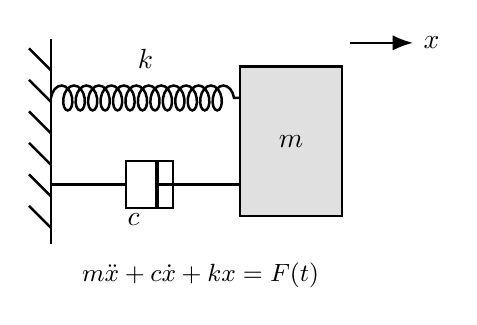
\begin{tikzpicture}[line width=0.9pt,>={Latex[length=2.6mm]}]
  % pared
  \draw[thick] (0,-1.3)--(0,1.3);
  \foreach \y in {-1.1,-0.7,...,1.1} \draw (0,\y)--(-0.28,\y+0.28);
  % resorte
  \draw[decorate,decoration={coil,aspect=0.6,segment length=4.5pt,amplitude=4.5pt}] (0,0.55)--(2.4,0.55);
  \node at (1.2,1.05){$k$};
  % amortiguador
  \draw (0,-0.55)--(0.95,-0.55);
  \draw (0.95,-0.85) rectangle (1.55,-0.25);
  \draw[line width=1.4pt] (1.35,-0.85)--(1.35,-0.25);
  \draw (1.35,-0.55)--(2.4,-0.55);
  \node at (1.05,-1.0){$c$};
  % masa
  \draw[thick,fill=black!12] (2.4,-0.95) rectangle (3.7,0.95);
  \node at (3.05,0){$m$};
  % desplazamiento
  \draw[->] (3.8,1.25)--(4.6,1.25) node[right]{$x$};
  \node at (1.9,-1.7){\small $m\ddot x+c\dot x+kx=F(t)$};
\end{tikzpicture}
\end{document}
